
\section{Logikk}
\begin{frame}{Proposisjoner}
\begin{itemize}
    \item En proposisjon er et uttrykk med en sannhetsverdi, som alltid er enten Sann (T) elller Usann (F).
    \item Ofte setter vi dem i variabler, for å gjøre det lettere å lese.
\end{itemize}
\begin{block}{Proposisjoner}
    p := 2 < 3 \\
    q := "Månen er laget av ost"\\
    r := "MNF130 er et nyttig fag for informatikere"
\end{block}
\begin{block}{Ikke proposisjoner}
    "Hva skal vi ha til middag i dag?"\\
    x + y < z
\end{block}
\end{frame}

\begin{frame}{$\lnot$, og sannhetstabeller}
\begin{itemize}
    \item Gitt en proposisjon $p$, kan vi representere den motsatte proposisjonen som $\lnot p$.
    \item Vi kan tegne opp alle mulige verdier et slikt uttrykk kan ha i en tabell.
\end{itemize}

\begin{block}
    La $p := 2 < 3$. \\
    $p$ = "Det er sant at 2 er mindre enn 3" \\
    $\lnot p$ = "Det er ikke sant at 2 er mindre enn 3"
\end{block}
\begin{tabular}{c|c}
$p$ & $\lnot p$ \\ \hline
T & F \\
F & T \\ \hline
\end{tabular}
\end{frame}

\begin{frame}{$\lor$ og $\land$}
    \begin{itemize}
        \item Vi kan slå sammen flere proposisjoner til et større uttrykk på mange forskjellige måter.
    \end{itemize}
    \begin{block}{Eksempel}
        La $p$ := Jorden er flat, og $q$ := Månen er flat\\
        $p \lor q$ = Jorden er flat \textbf{eller} månen er flat\\
        $p \land q$ = Jorden er flat \textbf{og} månen er flat\\
    \end{block}
    \begin{tabular}{c|c|c|c}
        $p$ & $q$ & $p \lor q$ & $p \land q$ \\ \hline
        T & T & T & T \\
        T & F & T & F \\
        F & T & T & F \\
        F & F & F & F \\
    \end{tabular}
\end{frame}

\begin{frame}{$\rightarrow$ og $\leftrightarrow$}
    \begin{itemize}
        \item En proposisjon kan implisere en annen proposisjon.
    \end{itemize}
    \begin{block}{Eksempel}
        La $p$ := "Det regner ute", og $q$ := "Bakken er våt"\\
        $p \rightarrow q$ = "Hvis det regner ute, blir bakken våt"\\
        $p \leftrightarrow q$ = "Det regnet ute hvis og bare hvis bakken er våt"
    \end{block}
    \begin{tabular}{c|c|c|c}
        $p$ & $q$ & $p \rightarrow q$ & $p \leftrightarrow q$ \\ \hline
        T & T & T & T \\
        T & F & F & F \\
        F & T & T & F \\
        F & F & T & T \\
    \end{tabular}
\end{frame}

\begin{frame}{Ekvivalenser og tautologier}
    \begin{itemize}
        \item Når to logiske uttrykk alltid har samme verdi, sier vi at de er \emph{logisk ekvivalente}.
        \item Om et uttrykk alltid er sant, uavhengig av innholdet, kaller vi det en tautologi.
    \end{itemize}
    \begin{tabular}{c|c|c|c}
         $p$ & $\lnot p$ & $\lnot \lnot p$ & $p \lor \lnot p$\\ \hline
         T & F & T & T\\
         F & T & F & T
    \end{tabular}
    \begin{itemize}
        \item Konklusjon 1: $p \equiv \lnot \lnot p$
        \item Konklusjon 2: $p \lor \lnot p \equiv T$, og er en tautologi
        \item For å se om to uttrykk er ekvivalente, tegn sannhetstabellen og se om kollonene deres er det samme.
        \item For å se om et uttrykk er en tautologi, tegn sannhetstabellen og se om kolonnen alltid er T.
    \end{itemize}
\end{frame}

\begin{frame}{Noen viktige logiske ekvivalenser}
    \begin{columns}
    \begin{column}{0.32\textwidth}
        \begin{tabular}{l|c}
        Ekvivalens & Navn \\ \hline
        $p \land T \equiv p$ & Identity\\
        $p \lor F \equiv p$ \\ \hline
        
        $p \lor T \equiv T$ & Domination\\
        $p \land F \equiv F$\\ \hline
        
        $p \lor p \equiv p$ & Idempotent\\
        $p \land p \equiv p$ \\ \hline
        
        $p \equiv \lnot \lnot p$ & Negation\\ \hline
        
        $p \lor q \equiv q \lor p$ & Commutative\\
        $p \land q \equiv q \land p$ \\
        

    \end{tabular}
    \end{column}
    \begin{column}{0.52\textwidth}
        \begin{tabular}{l|c}
        Ekvivalens & Navn \\ \hline
        
        $(p \lor q) \lor r \equiv p \lor (q \lor r)$ & Associative\\
        $(p \land q) \land r \equiv p \land (q \land r)$ \\ \hline
        
        $p \lor (q \land r) \equiv (p \lor q) \land (p \lor r)$ & Distributive\\
        $p \land (q \lor r) \equiv (p \land q) \lor (p \land r)$ \\ \hline
        
        $\lnot (p \land q) \equiv \lnot p \lor \lnot q$ & De Morgan \\
        $\lnot (p \lor q) \equiv \lnot p \land \lnot q$ \\ \hline
        
        $p \lor (p \land q) \equiv p$ & Absorption \\
        $p \land (p \lor q) \equiv q$ \\ \hline
        
        $p \lor \lnot p \equiv T$ & Negation \\
        $p \land \lnot p \equiv F$ \\
        \end{tabular}
    \end{column}
\end{columns}
\end{frame}

\begin{frame}{Flere viktige logiske ekvivalenser}
    \begin{columns}
    \begin{column}{0.48\textwidth}
        \begin{tabular}{c}
            Ekvivalenser med $\rightarrow$ \\ \hline
            $p \rightarrow q \equiv \lnot p \lor q$ \\
            $p \rightarrow q \equiv \lnot p \rightarrow \lnot q$ \\
            $p \lor q \equiv \lnot p \rightarrow q$ \\
            $p \land q \equiv \lnot (p \rightarrow \lnot q)$ \\
            $\lnot (p \rightarrow q) \equiv p \land \lnot q$ \\
            $(p \rightarrow q) \land (p \rightarrow r) \equiv p \rightarrow (q \land r)$ \\
            $(p \rightarrow q) \land (q \rightarrow r) \equiv (p \lor q) \rightarrow r$ \\
            $(p \rightarrow q) \lor (p \rightarrow r) \equiv p \rightarrow (q \lor v)$ \\
            $(p \rightarrow r) \lor (q \rightarrow r) \equiv (p \land q) \rightarrow r$
        \end{tabular}
    \end{column}
    \begin{column}{0.48\textwidth}
        \begin{tabular}{c}
            Ekvivalenser med $\leftrightarrow$ \\ \hline
            $p \leftrightarrow q \equiv p \rightarrow q \land q \rightarrow p$ \\
            $p \leftrightarrow q \equiv \lnot p \leftrightarrow \lnot q$ \\
            $p \leftrightarrow q \equiv (p \land q) \lor (\lnot p \land \lnot q)$\\
            $\lnot (p \leftrightarrow q) \equiv p \rightarrow \lnot q$
        \end{tabular}
    \end{column}
    \end{columns}
\end{frame}

\begin{frame}{Typisk logikkoppgave}
    \begin{columns}
    \begin{column}{0.48\textwidth}
        Vis at $(p \land \lnot q) \rightarrow \lnot r$ og $(p \land q) \rightarrow q$ er logisk ekvivalente, ved å bruke enkle logiske ekvivalenser.\\[1cm]
        
        1. $a \rightarrow b \equiv \lnot a \lor b$ \\
        2. $\lnot (a \land b) \equiv \lnot a \lor \lnot b$\\
        3. $\lnot (\lnot a) \equiv a$
    \end{column}
    \begin{column}{0.48\textwidth}
        \begin{math}
            (p \land q) \rightarrow \lnot r \\
            \equiv \lnot (p \land \lnot q) \lor \lnot r \\
            \equiv (\lnot p \lor \lnot \lnot q) \lor \lnot r \\
            \equiv (\lnot p \lor q) \lor \lnot r \\
            \equiv \lnot p \lor q \lor \lnot r \\
            \equiv \lnot p \lor \lnot r \lor q \\
            \equiv \lnot (p \land r) \lor q \\
            \equiv (p \land r) \rightarrow q
            \qed
        \end{math}
    \end{column}
    \end{columns}
\end{frame}

\begin{frame}{Predikater}
    \begin{itemize}
        \item Et predikat er bare en funksjon som returnerer T eller F.
        \item Gitt et predikat og riktig antall argumenter, kan vi evaluere det som en vanlig proposisjon.
    \end{itemize}
    \begin{block}{Eksempler på predikater}
        $P(x, y, z) = x + y < z$\\
        $Q(s)$ = $s$ contains $'a'$
    \end{block}
    \begin{block}{Eksempler på evaluering}
        $P(1, 2, 3) = 1 + 2 < 3 = 3 < 3 = F$ \\ 
        $Q("Steinar") = "Steinar"$ contains $'a' = T$
    \end{block}

\end{frame}

\begin{frame}{Kvantorer (/Quantifiers)}
    \begin{itemize}
        \item Ofte vil vi si noe om et predikat $P(x)$, men for flere potensielle $x$ samtidig.
        \item $\forall x P(x)$ = "For alle $x$ er det sant at $P(x)$"
        \item $\exists x P(x)$ = "Det eksisterer en $x$ slik at det er sant at $P(x)$"
    \end{itemize}
    
    \begin{block}{Eksempler}
        $\forall x (x < x + 1)$ = "For alle x er det sant at $x < x +1$"\\[5mm]
        $\exists x (x > x^2)$ = "Det eksisterer en x slik at det er sant at $x > x^2$"
    \end{block}
\end{frame}

\begin{frame}[fragile]{Kvantorer i praksis}
    \begin{minted}[fontsize=\scriptsize]{python}
def forall(p, xs):
    for x in xs:
        if not p(x):
            return False
    return True
    
def exists(p, xs):
    for x in xs:
        if p(x):
            return True
    return False
    \end{minted}
    
    \begin{itemize}
        \item exists(p, xs) = $\exists x (x \in xs \land p(x))$
        \item forall(p, xs) = $\forall x (x \in xs \land p(x))$
    \end{itemize}
\end{frame}

\begin{frame}{Nøstede kvantorer (/Nested quantifiers)}
    \begin{itemize}
        \item Ofte vil vi si noe om mange kombinasjoner av variabler samtidig.
        \item Da slå vi sammen flere $\forall$ og $\exists$.
    \end{itemize}
    
    \begin{block}{Eksempler}
        $\forall x \forall y ()$ \\
        $\forall x \exists y (x * y = 1)$ = "For alle x eksisterer det en y slik at er $x * y = 1$" \\
        $\exists x \forall y (x^2 < y^2)$ = "Det eksisterer en x slik at for alle y er $x^2 < y^2$"\\
        $\lnot \exists n \exists a \exists b \exists c (a,b,c,n \in Z \land n > 2 \land a^n + b^n = c^n)$
    \end{block}
\end{frame}

\begin{frame}{De Morgan dukker opp igjen}
Det viser seg at De Morgan's lover også fungerer på kvantorer.
    \begin{itemize}
        \item $\lnot \forall x P(x) \equiv \exists x \lnot P(x)$
        \item $\lnot \exists x P(x) \equiv \forall x \lnot P(x)$
    \end{itemize}
    \begin{columns}
    \begin{column}{0.48\textwidth}
        
\includegraphics[scale=1]{bigger fish.PNG}
    \end{column}
    \begin{column}{0.48\textwidth}
        
\includegraphics[scale=0.3]{Always a bigger fish.jpeg}
    \end{column}
    \end{columns}
    

\end{frame}

\subsection*{Spørretid}
\begin{frame}{Spørsmål?}
    \begin{figure}
        \centering
        
\includegraphics[height = 4.9cm]{images/guillaume5.jpg}
        \caption{Guillaume på Vidden}
        \label{fig:guillaume5}
    \end{figure}
\end{frame}

\section{Mengdelære og funksjoner}
\begin{frame}{Sett / Mengder}
    Et sett, eller en mengde, er en kolleksjon av objekter med to regler:\\
    \indent \hspace{3mm}    1. Det inneholder ingen duplikater\\
    \indent \hspace{3mm}    2. Det har ingen konkret rekkefølge
    
    \begin{block}{Eksempel}
        Alle de følgende settene er like: \\
        $\{1, 2, 3\}$, $\{3, 2, 1\}$ \\
        $\{1, 1, 1, 1, 2, 2, 3, 3\}$
    \end{block}
    
    \begin{block}{Eksempel}
        $1 \in \{1, 2, 3\}$ = T \\
        $5 \in \{1, 2, 3\}$ = F
    \end{block}
\end{frame}


\begin{frame}{Kjente sett}
    Flere sett bruker vi veldig ofte. Her er noen av dem.
    
    \begin{tabular}{c|l|c}
        Symbol & Navn & Innhold \\
        $\mathbb{N}$ & Naturlige tall & $\{0, 1, 2, 3, ....\}$\\
        $\mathbb{Z}$ & Heltall & $\{... -2, -1, 0, 1, 2, 3, ....\}$\\
        $\mathbb{Q}$ & Rasjonale tall & $\{-3/2, 1/10, 4/5, 5/4, ....\}$\\
        $\mathbb{R}$ & Reelle tall & $\{\pi, e, 0.111111111..., 2*\pi, .....\}$\\
        $\emptyset$ & Det tomme settet & $\{\}$
    \end{tabular}
    
\end{frame}

\begin{frame}{Settbyggingsnotasjon}
    Istedet for å manuelt skrive opp alle elementene i et sett, eller å bruke uformell \enquote{...}-notasjon, kan vi bruke setbyggingsnotasjon.
    \begin{block}{Eksempler}
        $\{ n | n \in \mathbb{N}\}$ = $\mathbb{N}$\\
        $\{ n \cdot 2 | n \in \mathbb{N}\}$ = $\{0, 2, 4, 6, 8, ....\}$\\
        $\{ i / 2 | i \in \mathbb{N}, i$ mod $3 = 0\}$ = $\{0, 1.5, 3, 4.5, 6, ...\}$
    \end{block}
\end{frame} 

\begin{frame}{$\cup$, $\cap$, $\bar{}$ og $-$}
    $A \cup B := \{x | x \in A \lor x \in B\}$ \\
    $A \cap B := \{x | x \in A \land x \in B\}$\\
    $A - B = A \backslash B := \{x | x \in A\land  x \notin B\}$\\
    $A^C = \bar{A} := \{x | x \notin A\}$
    

    \begin{figure}%
        \centering
        \subfloat[\centering $A \cup B$]{{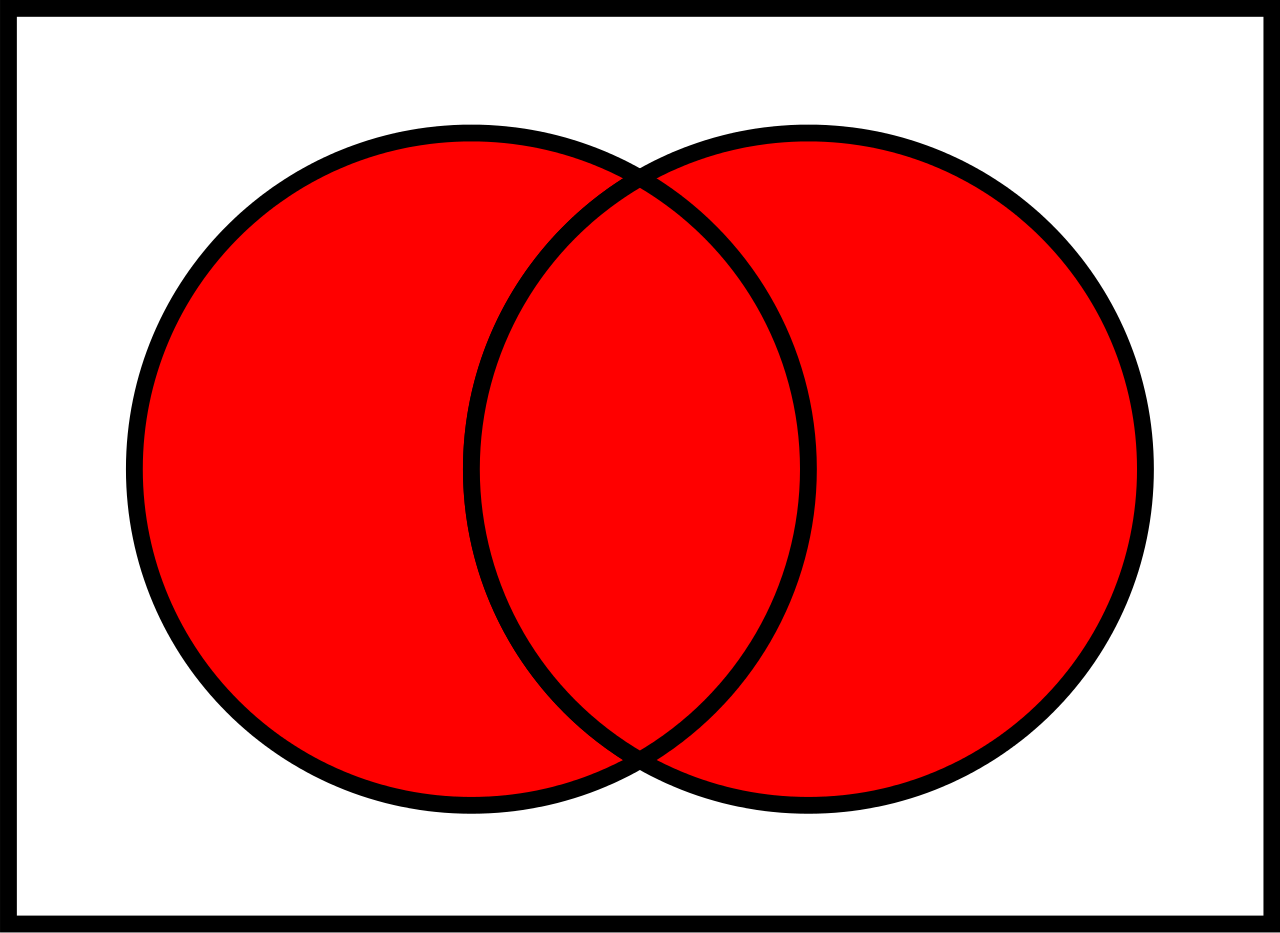
\includegraphics[width=2.5cm]{union.png} }}%
        \qquad
        \subfloat[\centering $A \cap B$]{{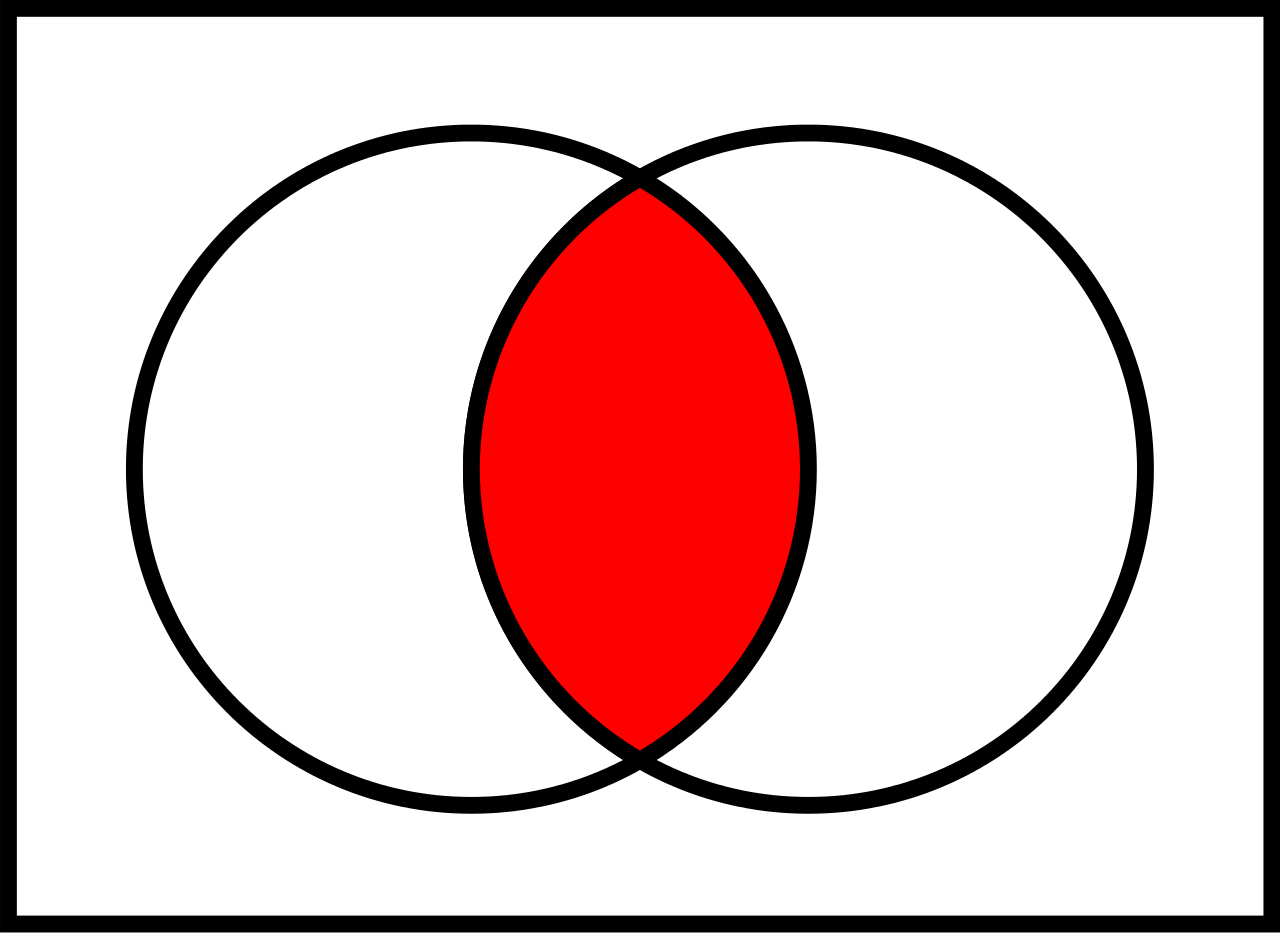
\includegraphics[width=2.5cm]{snitt.png} }}%
        \qquad
        \subfloat[\centering $B - A$]{{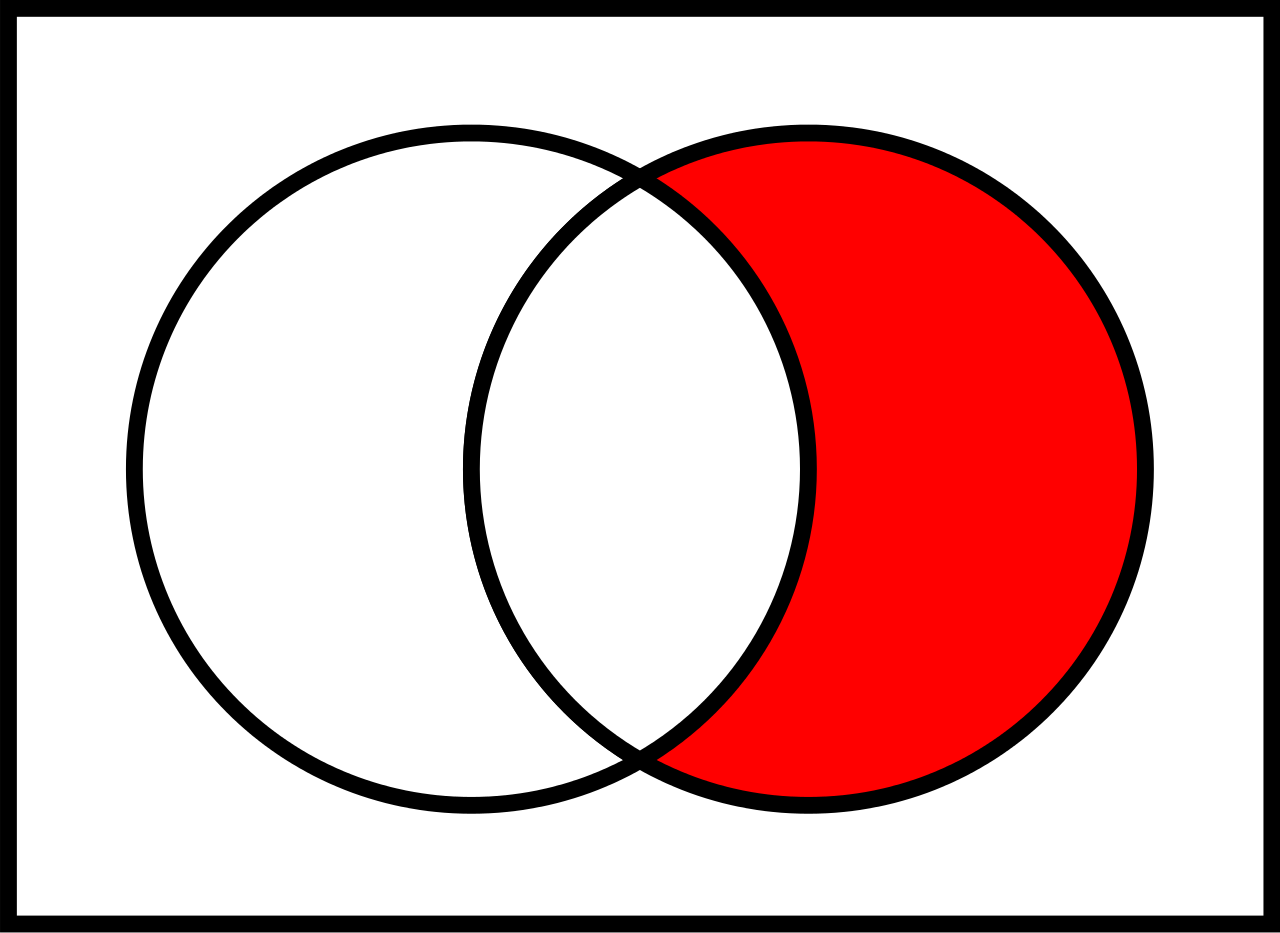
\includegraphics[width=2.5cm]{minus.png} }}%
        \qquad
        \subfloat[\centering $\bar{A}$]{{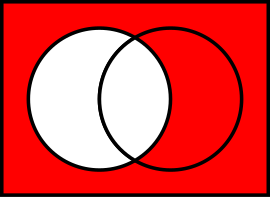
\includegraphics[width=2.5cm]{complement.png} }}%
        % \caption{Vennediagramer}%
        \label{fig:example2}%
    \end{figure}
\end{frame}

\begin{frame}{$\subset, \subseteq, =, \supseteq, \supset$}
    Vi har flere måter å uttrykke at et sett inneholder elementer fra et annet sett.
    \begin{itemize}
        \item $A \subseteq B := \forall x (x \in A \rightarrow x \in B)$
        \item $A \supseteq B := B \subseteq A$
        \item $A \subset B := \forall x (x \in A \rightarrow x \in B) \land \exists y (y \in B \land y \notin A)$
        \item $A \supset B := B \subset A$
        \item $A = B := A \subseteq B \land B \subseteq A$
    \end{itemize}
    
    \begin{block}{Eksempler}
        $\{1\} \subseteq \{1, 2\}$ = T\\
        $\{1\} \subseteq \{5\}$ = F\\
        $\{a, b\} \subset \{a, b\}$ = F\\
        $\{a, b\} \subseteq \{a, b\}$ = T
    \end{block}
    
\end{frame}

\begin{frame}{Tavleoppgaver fra H19}
    \begin{itemize}
        \item Vis eller motbevis at $(A - C) \cap (B - C) = \emptyset.$
        \item Vis eller motbevis at $(A - C) \cap (C - B) = \emptyset.$
    \end{itemize}
    
    For å løse det med vennediagrammer:
    \begin{itemize}
        \item Tegn et vennediagram. Begynn med sirkler for A, B, etc.
        \item Farg inn (helst med forskjellige farger) områdene til deluttrykkene, dvs $(A - C)$ eller $(B - C)$ i dette eksemplet.
        \item Bruk områdene i deluttrykkene til å farge omårdene i de større uttrykkene, dvs hele $(A - C) \cap (B - C)$ her.
        \item Er områdene til hele uttrykkene på hver side av = det samme?
    \end{itemize}
    Alternativt: bruk definisjonene til $\cap$, $\cup$, etc til å omformulere uttrykket til det på høyresiden av =.
\end{frame}

\begin{frame}{Nyttige regler for sett}
        \begin{tabular}{l|c}
        Ekvivalens & Navn \\ \hline
        $A \cap U = A$ & Identity\\
        $A \cup \emptyset = A$ \\ \hline
        
        $A \cup U = U$ & Domination\\
        $A \cap \emptyset = \emptyset$\\ \hline
        
        $A \cup A = A$ & Idempotent\\
        $A \cap A = A$ \\ \hline
        
        $A = (A^C)^C$ & Negation\\ \hline
        
        $A \cup B = B \cup A$ & Commutative\\
        $A \cap B = B \cap A$ \\

    \end{tabular}
    \hfill
        \begin{tabular}{l|c}
        Ekvivalens & Navn \\ \hline
        
        $(A \cup B) \cup C = A \cup (B \cup C)$ & Associative\\
        $(A \cap B) \cap C = A \cap (B \cap C)$ \\ \hline
        
        $A \cup (B \cap C) = (A \cup B) \cap (A \cup C)$ & Distributive\\
        $A \cap (B \cup C) = (A \cap B) \cup (A \cap C)$ \\ \hline
        
        $(A \cap B)^C = A^C \cup B^C$ & De Morgan \\
        $(A \cup B)^C = A^C \cap B^C$ \\ \hline
        
        $A \cup (A \cap B) = A$ & Absorption \\
        $A \cap (A \cup B) = A$ \\ \hline
        
        $A \cup A^C = U$ & Negation \\
        $A \cap A^C = \emptyset$ \\
        \end{tabular}
\end{frame}

\begin{frame}{Funksjoner}
    Funksjoner kjenner vi fra INF100 i fjor. Nå skal vi formalisere dem litt mer.\\
    Se på funksjoner som en utregning fra et eller flere sett til et annet sett.\\
    Domenet til en funksjon er inputsettet.\\
    Kodemenet til en funksjon er outputsettet.\\
    %\begin{block}
    \begin{columns}
    \begin{column}{0.28\textwidth}
         $f : \mathbb{R} \rightarrow \mathbb{R}$\\
        $f(x) := x+1$ \\
        $g : \mathbb{Z} \rightarrow Bool$ \\
        $P : (\mathbb{R}, \mathbb{R}) \rightarrow Bool$\\
        $P(x, y) := x^2 < y$
     \end{column}
    \begin{column}{0.28\textwidth}
         $$
            g(n) :=
            \begin{cases}
            T, n \text{ mod } 2 = 0\\
            F, \text{otherwise}\\
            \end{cases}
        $$
    \end{column}
       
       
        
    \end{columns}
    %\end{block}
\end{frame}

\begin{frame}{Injektivitet, Surjektivitet}
    En funksjon $f : A \rightarrow B$ er:
    \begin{itemize}
        \item Injektiv hvis $\forall a_1 \forall a_2 (f(a_1) = f(a_2) \rightarrow a_1 = a_2)$.     Med andre ord: alle inputs gir et unikt output.\\
        \item Surjektiv hvis $\forall b \exists a (f(a) = b)$. Med andre ord: alle $b$ har minst én representant i $A$.
        \item Bijektiv hvis den er både injektiv og surjektiv. Da har den et invers.
    \end{itemize}
    \begin{figure}%
        \centering
        \subfloat[\centering $Injektiv$]{{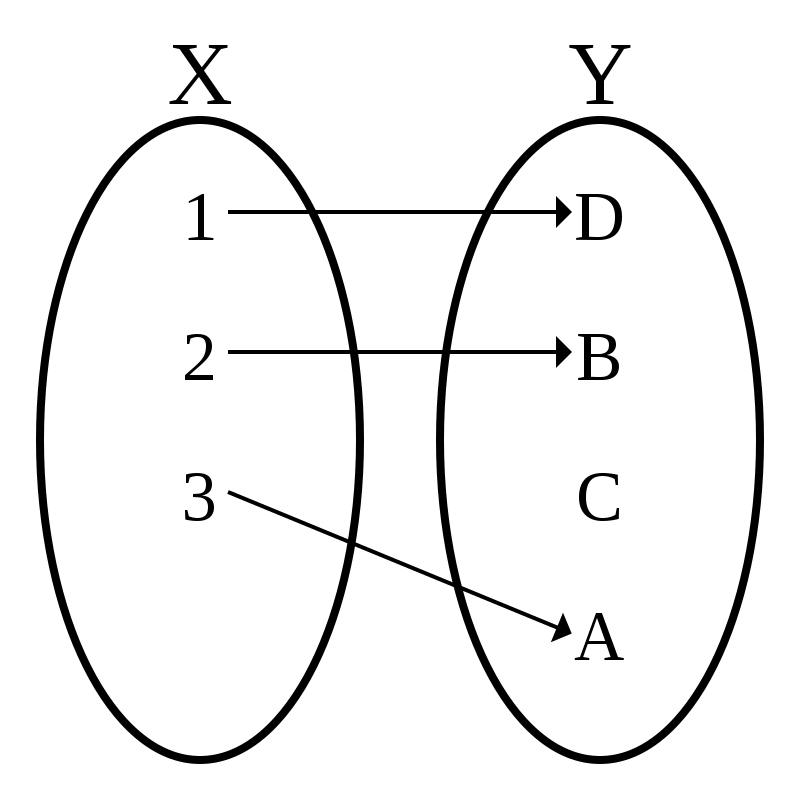
\includegraphics[width=2.5cm]{inj.png} }}%
        \qquad
        \subfloat[\centering $Surjektiv$]{{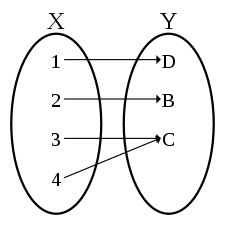
\includegraphics[width=2.5cm]{sur.png} }}%
        \qquad
        \subfloat[\centering $Bijektiv$]{{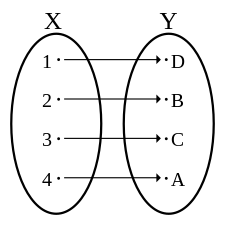
\includegraphics[width=2.5cm]{bi.png} }}%
        \qquad
        \subfloat[\centering $Ingenting$]{{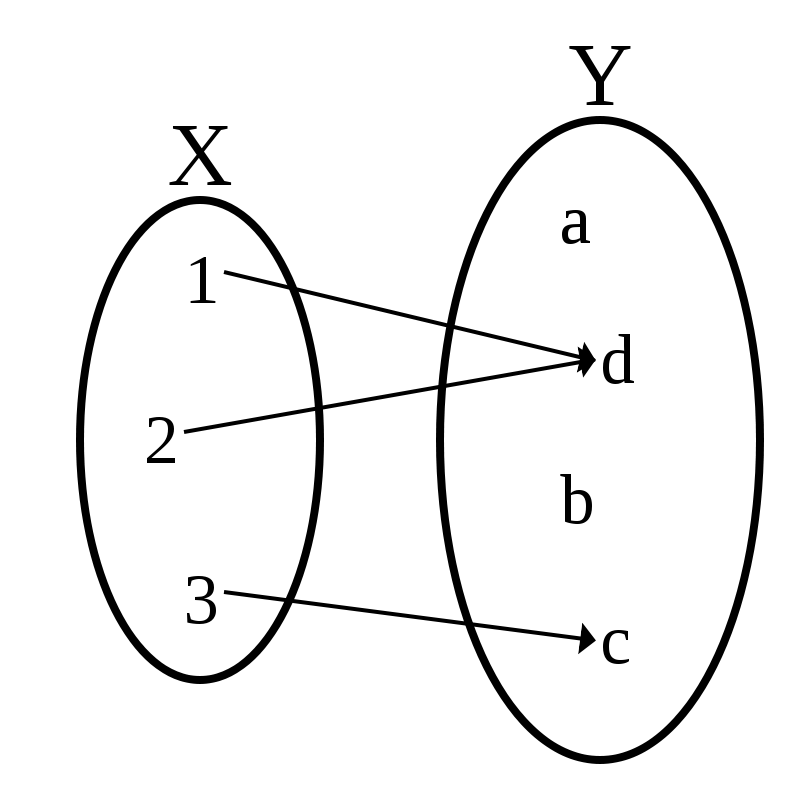
\includegraphics[width=2.5cm]{nothing.png} }}%
        \label{fig:example1}%
    \end{figure}
\end{frame}

\begin{frame}{Injektivitet, Surjektivitet}
    \begin{itemize}
        \item Injektiv:  $\forall a_1 \forall a_2 (f(a_1) = f(a_2) \rightarrow a_1 = a_2)$.\\
        \item Surjektiv: $\forall b \exists a (f(a) = b)$.\\
        \item Bijektiv: begge de over \\
    \end{itemize}
    
    \begin{block}{Avgjør om de følgende funksjonene er injektive, surjektive, eller bijektive:}
        $f : \mathbb{R} \rightarrow \mathbb{R}$, $f(x) := 2x + 1$\\
        $g : \mathbb{Z} \rightarrow \mathbb{Z}$, $g(x) := x$ mod $2$\\
        $h : \mathbb{R} \rightarrow \mathbb{R}$, $h(x) := e^x$\\
        $k : \mathbb{R} \rightarrow \mathbb{R^+}$, $k(x) := e^x$\\
    \end{block}
\end{frame}

\begin{frame}{Funksjonskomposisjon}
    \begin{columns}
    \begin{column}{0.5\textwidth}
Gitt to funksjoner:
    \begin{itemize}
        \item $f : A \rightarrow B$
        \item $g : B \rightarrow C$
    \end{itemize}
Kan vi definere en unik tredje funksjon: \\
    $g \circ f : A \rightarrow C$\\
    $g \circ f := g(f(x))$\\
Om en funksjon $f : A \rightarrow B$ er bijektiv, finnes det en unik invers funksjon $f^{-1} : B \rightarrow A$ slik at $f(f^{-1}(x)) = x$ og $f^{-1}(f(x)) = x$.
    \end{column}
    \begin{column}{0.33\textwidth}
    \begin{figure}
       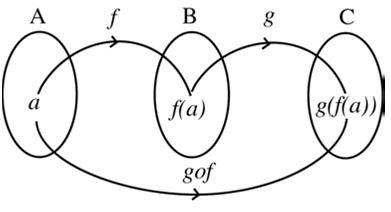
\includegraphics[scale = 0.4]{gof.jpeg} 
    \end{figure}
        
    \end{column}
    \end{columns}
\end{frame}

\begin{frame}{Kardinalitet}
    Om $A$ er et sett, er $|A|$ antall elementer i settet, \textit{kardinaliteten}, eller \textit{lengden}.\\
    To sett har samme kardinalitet om de har samme lengde. Da finnes det en bijeksjon mellom settene.
    \begin{block}
        $|\{a, b, c\}| = 3$\\
        $|\{\}| = 0$\\
        $|\mathbb{N}| = \aleph_0$
    \end{block}
\end{frame}

\begin{frame}{Tellbarhet}
    \begin{columns}
    \begin{column}{0.48\textwidth}
        Hva er størst av $|\mathbb{N}|$ og $|\mathbb{Z}|$?\\
        f(n) :=
        \begin{cases}
            \frac{n}{2}, n \text{ mod } 2 = 0\\
            -\frac{n+1}{2}, \text{otherwise}\\
        \end{cases}\\
        Konklusjon: $|\mathbb{N}|$ = $|\mathbb{Z}|$ = $\aleph_0$.
    \end{column}
    \begin{column}{0.48\textwidth}
        Hva er størst av $|\mathbb{N}|$ og $|\mathbb{Q}|$?\\
        $f(0) := 1$\\
        $f(n) := \frac{1}{2\lfloor f(n-1) \rfloor - f(n-1)+1}$\\
        $g(0) := 0$\\
        $g(2n) := f(n)$\\
        $g(2n-1) := -f(n)$\\
        Konklusjon: $|\mathbb{N}|$ = $|\mathbb{Q}|$ = $\aleph_0$
    \end{column}
    \end{columns}
    
    
    \newline Derimot er $|\mathbb{R}| > |\mathbb{N}|$. For en enkel forklaring med et eksempel, se Veritasiums video om Hilberts Hotell: \url{https://www.youtube.com/watch?v=OxGsU8oIWjY}
    
%Gud, alle disse feilmeldingene, Steinar
\end{frame}

\subsection*{Spørretid}
\begin{frame}{Spørsmål?}
    \begin{figure}
        \centering
        
\includegraphics[height = 4.9cm]{images/guillaume4.jpg}
        \caption{Guillaume på Vidden}
        \label{fig:guillaume4}
    \end{figure}
\end{frame}

\section{Relasjoner}
\begin{frame}[fragile]{Relasjoner}
    En relasjon fra $A$ til $B$ er et subset av $A \times B$.\\
    De er lettere å visualisere ved å tegne dem:\\
    
    R := $\{(a, b), (b, b), (d, c), (d, b), (a, c)\}$\\
\begin{tikzcd}
a \arrow[rr] \arrow[rrdd] &  & b \arrow[loop, distance=2em, in=305, out=235] \\
                          &  &                                               \\
d \arrow[rr] \arrow[rruu] &  & c                                            
\end{tikzcd}

Veldig ofte er $A$ og $B$ det samme, dvs et subset av $A \times A$. Da kaller vi det en relasjon \emph{på} $A$.
\end{frame}

\begin{frame}[fragile]{Praktisk eksempel på en relasjon}
    La objektene være alle typer i Python. \\
    La det være en relasjon fra $a$ til $b$ om det finnes en funksjon fra typen $a$ til typen $b$.\\
    
\begin{tikzcd}
Int \arrow[rr, "bool()", bend right] \arrow[dd, "str()", bend left] &  & Bool \arrow[lldd, "str()"] \arrow[ll, "int()"', bend right] \\
                                                                    &  &                                                             \\
Str \arrow[rr, ".split()"] \arrow[uu, "int()", bend left]           &  & {[Str]}                                                    
\end{tikzcd}
\end{frame}

\begin{frame}{Forskjellige typer relasjoner}
Gitt en relasjon $R \subseteq A \times A$ på $A$ har vi 5 viktige begreper for å beskrive den:
    \begin{itemize}
        \item Refleksiv: $\forall a ((a, a) \in R)$
        \item Symmetrisk: $\forall a \forall b ((a, b) \in R \leftrightarrow (b, a) \in R)$
        \item Antisymmetrisk: $\forall a \forall b ((a, b) \in R \rightarrow a = b)$
        \item Transitiv: $\forall a \forall b \forall c [(a, b) \in R \land (b, c) \in R \rightarrow (a, c) \in R]$\\

        \item Om en relasjoner er refleksiv, symmetrisk og transitiv, kaller vi det en ekvivalensrelasjon.
    \end{itemize}   
\end{frame}

\begin{frame}[fragile]{Refleksive relasjoner}
En relasjon $R$ er refleksive hvis $\forall a ((a, a) \in R)$.\\
    \begin{columns}
        \begin{column}{0.3\textwidth}
        Ikke refleksiv:
            \begin{tikzcd}
a \arrow[dd] \arrow[rr] &  & b                                             \\
                        &  &                                               \\
c \arrow[rruu]          &  & d \arrow[loop, distance=2em, in=305, out=235]
\end{tikzcd}
        \end{column}
        \begin{column}{0.3\textwidth}
Refleksiv:
\begin{tikzcd}
a \arrow[dd] \arrow[rr] \arrow[loop, distance=2em, in=305, out=235] &  & b \arrow[loop, distance=2em, in=305, out=235] \\
                                                                    &  &                                               \\
c \arrow[rruu] \arrow[loop, distance=2em, in=305, out=235]          &  & d \arrow[loop, distance=2em, in=305, out=235]
\end{tikzcd}
        \end{column}
    \end{columns}
\end{frame}

\begin{frame}[fragile]{Symmetriske relasjoner}
En relasjon $R$ er symmetrisk hvis $\forall a \forall b ((a, b) \in R \leftrightarrow (b, a) \in R)$.\\
    \begin{columns}
        \begin{column}{0.3\textwidth}
            Ikke symmetrisk:\\
            \begin{tikzcd}
a \arrow[dd]   &  & b                                             \\
               &  &                                               \\
c \arrow[rruu] &  & d \arrow[loop, distance=2em, in=305, out=235]
\end{tikzcd}
        \end{column}
        \begin{column}{0.3\textwidth}
        Symmetrisk:
        \begin{tikzcd}
a \arrow[dd, bend left]                          &  & b \arrow[lldd, bend right]                    \\
                                                 &  &                                               \\
c \arrow[rruu, bend right] \arrow[uu, bend left] &  & d \arrow[loop, distance=2em, in=305, out=235]
\end{tikzcd}
        \end{column}
    \end{columns}
\end{frame}

\begin{frame}[fragile]{Antisymmetriske relasjoner}
En relasjon $R$ er antisymmetrisk hvis $\forall a \forall b ((a, b) \in R \rightarrow a = b)$.\\
    \begin{columns}
        \begin{column}{0.3\textwidth}
        Ikke antisymmetrisk:
        \begin{tikzcd}
a \arrow[dd, bend left]                          &  & b \arrow[lldd, bend right]                    \\
                                                 &  &                                               \\
c \arrow[rruu, bend right] \arrow[uu, bend left] &  & d \arrow[loop, distance=2em, in=305, out=235]
\end{tikzcd}
        \end{column}
        \begin{column}{0.3\textwidth}
Antisymmetrisk:
\begin{tikzcd}
a                         &  & b                                             \\
                          &  &                                               \\
c \arrow[rruu] \arrow[uu] &  & d \arrow[loop, distance=2em, in=305, out=235]
\end{tikzcd}
        \end{column}
    \end{columns}
\end{frame}

\begin{frame}[fragile]{Transitive relasjoner}
En relasjon $R$ er transitiv om $\forall a \forall b \forall c [(a, b) \in R \land (b, c) \in R \rightarrow (a, c) \in R]$.\\
    \begin{columns}
        \begin{column}{0.3\textwidth}
        Ikke transitiv:
        \begin{tikzcd}
a \arrow[rr] &  & b \arrow[dd] \\
             &  &              \\
c            &  & d \arrow[ll]
\end{tikzcd}
        \end{column}
        \begin{column}{0.3\textwidth}
Transitiv:
\begin{tikzcd}
a \arrow[rr] \arrow[rrdd] \arrow[dd] &  & b \arrow[dd] \arrow[lldd] \\
                                     &  &                           \\
c                                    &  & d \arrow[ll]             
\end{tikzcd}
        \end{column}
    \end{columns}
\end{frame}

\begin{frame}{Tavleoppgaver om relasjoner}
Avgjør om følgende relasjoner er refleksive, symmetriske, anti-symmetriske, eller transitive:\\
    \begin{itemize}
        \item $R := \{(a, b) | a, b \in \mathbb{N}, a < b\}$
        \item $Q := \{(a, b) | a, b \in \mathbb{N}, a \leq b\}$
        \item $B_{p, q}$ := settet av alle logiske uttrykk gitt av $p$ og $q$\\
              $P := \{(a, b) | a, b \in B_{p, q}, a \equiv b\}$
        \item $S := \emptyset$
    \end{itemize}
\end{frame}

\subsection*{Spørretid}
\begin{frame}{Spørsmål?}
    \begin{figure}
        \centering
        
\includegraphics[height = 4.9cm]{images/guillaume3.jpg}
        \caption{Guillaume et sted Lukas ikke husker}
        \label{fig:guillaume3}
    \end{figure}
\end{frame}

\section{Bevis}

\begin{frame}{Beviser}
    Svært mange bevisoppgaver er på formen "Vis at $p \rightarrow q$".\\
    
    Om oppgaven er "Vis at om $n$ er et heltall og og $3n+2$ er et oddetall, da er $n$ et oddetall.", da er \\
    $p = $ "$n$ er et heltall og og $3n+2$ er et oddetall" \\
    $q = $ "$n$ er et oddetall"\\
    
Vi har mange teknikker for løse slike oppgaver. Problemet er at det ikke er opplagt hvilke som kan brukes. Det er bare å prøve seg frem.
\end{frame}

\begin{frame}{Direkte bevis}
    Et direkte bevis for $p \rightarrow q$ er et som antar at $p$ = T, og viser at det medfører at $q$ = T.\\
    Dette er ofte de enkleste bevisene. Om du ikke vet hva slags teknikk som skal brukes, forsøk denne først.\\
    
    \begin{block}{Vis at om $x$ og $y$ er partall, da er $x + y$ også et partall.}
        Vi antar først at $x$ og $y$ er partall. Da kan vi omskrive dem:\\
        $x = 2a$, $y = 2b$, for $a, b \in \mathbb{Z}$.\\
        Da er $x + y = 2a + 2b = 2(a + b)$.\\
        Siden vi ganger med $2$ blir $2(a + b)$ et partall uavhengig av hva $a + b$ er.
        \qed
    \end{block}
\end{frame}

\begin{frame}{Kontrapositivt bevis (/proof by contraposition)}
    Istedet for å bevise $p \rightarrow q$, er det ofte lettere å bevise $\lnot q \rightarrow \lnot p$. De uttrykkene er helt ekvivalente.\\
    Det vil si å anta at $q = F$, og vise at da må også $p$ = F.\\
    
    \begin{block}{Vis at for $a, b \in \mathbb{Z}$, vil $a + b \geq 15$ medføre at $a \geq 8 \lor b \geq 8$.}
        La oss vise det motsatte: at om $a <8 \land b < 8$, er $a + b < 15$.\\
        Da er $a \leq 7$ og $b \leq 7$, og\\
        $a + b \leq 7 + 7$\\
        $a + b \leq 14$\\
        $a + b < 15$
        \qed
    \end{block}
\end{frame}

\begin{frame}{Motsigelsesbevis (/proof by contradiction)}
    For å bevise en proposisjon $p$, kan det vi heller bevise at $\lnot p$ leder til en motsigelse. Det vil si, motbevis det motsatte.
    
    \begin{block}{Vis at summen av et rasjonalt tall $\frac{a}{b}$ og et irrasjonalt tall $c$ også er et irrasjonalt tall.}
    Vi antar det motsatte: at summen blir et rasjonalt tall: $\frac{a}{b}$ + $c$ = $\frac{e}{d}$ for $e, d \in \mathbb{Z}$.\\
    $\implies \frac{e}{d} - \frac{a}{b} = c$\\
    $\implies \frac{b\cdot d - a \cdot d}{b\cdot d} = c$\\
    Men det impliserer at $c$ er et rasjonalt tall, som er en selvmotsigelse. Derfor er det usant at summen er et rasjonalt tall, som betyr at summen må være irrasjonal. 
    \qed
    
    \end{block}
\end{frame}

\begin{frame}{Uttømmende bevis (/proof by exhaustion)}
    Noen ganger orker vi ikke finne på et elegant bevis. Da tar vi heller for oss hvert enkelt tilfelle hver for seg, og når vi har vist at det holder for alle tilfeller har vi bevist påstanden. \\
    
    \begin{block}{Vis at alle sommer-OL har blitt arrangert i årstall delelige på 4.}
        1896 mod 4 = 0 \checkmark \\
        1900 mod 4 = 0 \checkmark \\
        1904 mod 4 = 0 \checkmark \\
        .... \\
        (de neste 24 linjene er trivielle og etterlatt som en oppgave for leseren)\\
        ....\\
        2020 mod 4 = 0 \checkmark
    \end{block}
\end{frame}

\begin{frame}{Motbeviser}
    For å bevise at en påstand er usann, holder det vanligvis bare å finne et moteksempel. Dette er vanligvis den letteste typen bevis.
    
    \begin{block}{Påstand: det er ikke mulig å plassere 8 dronninger på et sjakkbrett uten at noen av dem truer hverandre.}
    \begin{figure}
        \centering
        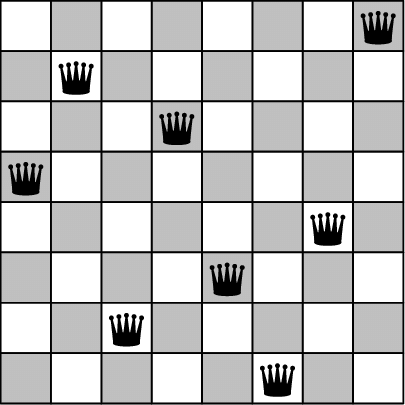
\includegraphics[scale=0.20]{8 queens.png}
        % \caption{Motbevis}
        \label{fig:my_label}
    \end{figure}
    
    \end{block}
\end{frame}

\subsection{Induksjon}
\begin{frame}
TODO: Fill with content @Steinar 
% Wadde Hadde Dudde Da
\end{frame}

\subsection{Relasjoner}
\begin{frame}
TODO: Fill with content @Steinar 
\end{frame}

\subsection*{Spørretid}
\begin{frame}{Spørsmål?}
    \begin{figure}
        \centering
        
\includegraphics[height = 4.9cm]{images/guillaume7.jpg}
        \caption{Guillaume på Blåmanen}
        \label{fig:guillaume7a}
    \end{figure}
\end{frame}

\section{Sekvenser/Rekker}
\begin{frame}

TODO: Fill with content @Steinar 
\end{frame}

\subsection*{Spørretid}
\begin{frame}{Spørsmål?}
    \begin{figure}
        \centering
        
\includegraphics[height = 4.9cm]{images/guillaume7.jpg}
        \caption{Guillaume, wait, dette bildet hadde vi før?}
        \label{fig:guillaume7b}
    \end{figure}
\end{frame}